%!TEX root = report.tex
\subsection*{Particle in a box}
\begin{itemize}
    % \item \sout{Plot solution to matrix problem, eigenfunctions $\psi_n$ against exact solution eq. (2.10) and eigenvalues $\lambda_n$ against exact result $(\pi n)^2$}
    \item \hl{Introduce measure of error between numerical eigenfunctions and exact result and investigate how it scales with discretization step $\Delta x$}
    % \item \sout{Plot state of system as function of time with different initial conditions}
    % \item \sout{Use/discuss use of delta function as initial condition}
\end{itemize}

In \cref{fig:box_solutions} the numerically estimated eigenvalues (left) and eigenfunctions (right) are plotted together with the exact results from \cref{eq:exact_eigenfunctions}, for an infinite well with $\Delta x' = 1/200$. We see that the eigenfunction match the analytical solution perfectly, but that there is some discrepancy in the eigenvalues at $n$ greater than approx. 30.

\begin{figure}[ht!]%
\centering%
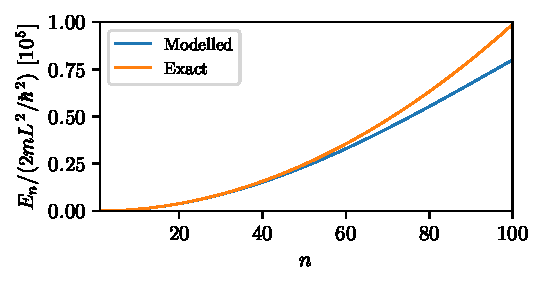
\includegraphics{figs/box_eigenvalues.pdf}\\%
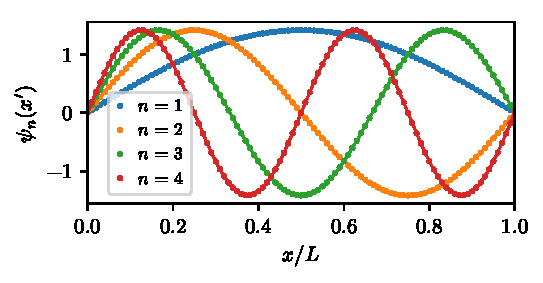
\includegraphics{figs/box_eigenvectors.pdf}%
\caption{Eigenvalues (top) and eigenfunctions (bottom) in an infinite well with $\Delta x' = 1/200$. \label{fig:box_solutions}}%
\end{figure}

In \cref{fig:box_time_psi0} the time development of the particle in a box is plotted for the initial condition $\Psi_0 = \psi_0$, the first eigenfunction.

\begin{figure}[ht!]%
\centering%
% 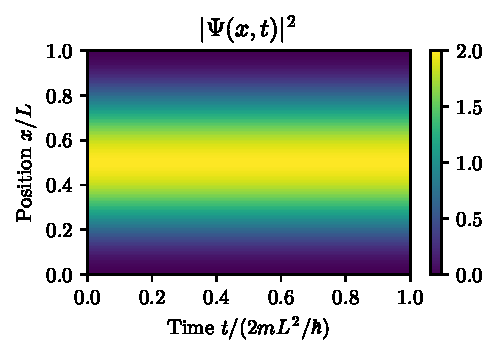
\includegraphics{figs/box_psi0_prob.pdf}\\%
% 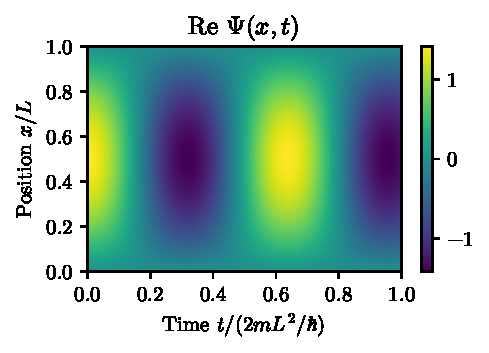
\includegraphics{figs/box_psi0_real.pdf}%
% 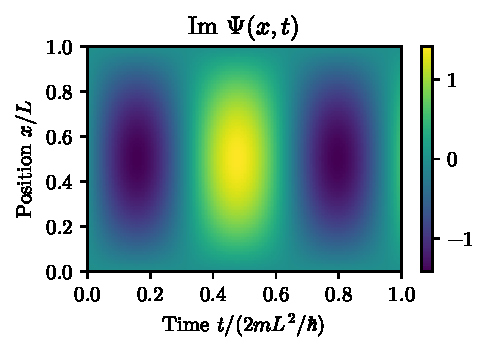
\includegraphics{figs/box_psi0_imag.pdf}%
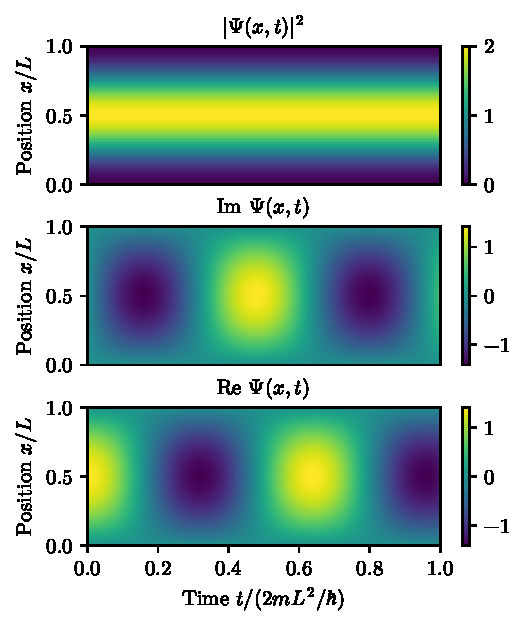
\includegraphics{figs/box_psi0.pdf}% single figure
\caption{Time-development of particle in a well with initial condition $\Psi_0(x',t'=0) = \psi_0$ and $\Delta x' = 1/200$ and $\Delta t' = 1/2000$. \label{fig:box_time_psi0}}%
\end{figure}

Using a delta function as initial condition $\Psi_0(x) = \delta(x - 1/2)$ fixes the initial position of the particle at $x=1/2$. This results in coefficients
\begin{equation}
    \alpha_n = \int \psi_n^{*}(x)\delta(x - 1/2) \dif x = \psi_n^{*}(x=1/2),
\end{equation}
which means that the initial wave function will be a combination of all eigenfunctions $\psi_n$'s. To properly represent this we need to include an infinite number of eigenfunctions. Further, since we have an exact position (with \emph{infinite certainty}) means that we have \emph{infinite uncertainty} in the momentum of the particle, following the uncertainty princinple. This means that any results for $t>0$ will not make any sense. Now, the numerical simulations doesn't know that this is not possible, so it willingly spits out results like the ones in \cref{fig:box_time_deltaf}. The simulations can not use an infinite number of eigenfunctions to represent the initial condition, so in practice we are probably seeing the results of using a bad approximation of a triangle wave or a Gaussian as initial condition.

\begin{figure}[ht!]%
\centering%
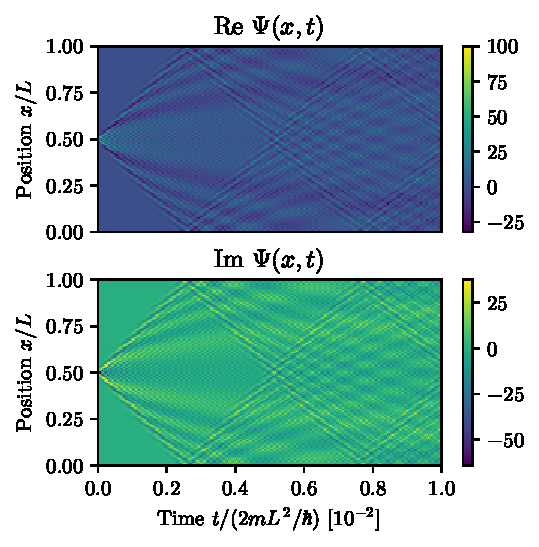
\includegraphics[width=0.49\textwidth]{figs/box_deltaf.pdf}%
\caption{Time-development of particle in a well with initial condition $\Psi_0(x',t'=0) = \delta(x' - 1/2)$ and $\Delta x' = 1/200$ and $\Delta t' = 10^{-5}$. \label{fig:box_time_deltaf}}%
\end{figure}

\subsection*{Double well}
In \cref{fig:double_well_solutions} we have plots of the first three eigenfunctions of the double well (right), and the first eigenvalues. We see that the first excited state ($n=2$) has nearly the same wave function as the ground state, but with odd parity (the blue line for $n=1$ is hidden under the orange line for $n=2$ in the left half of the plot).
\begin{figure}[ht!]%
\centering%
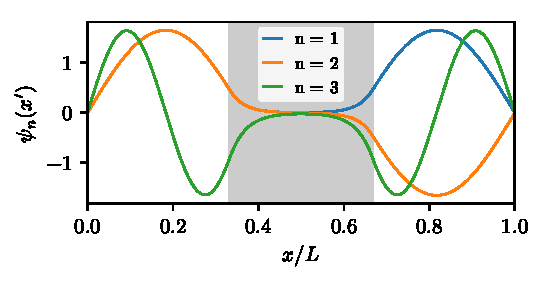
\includegraphics{figs/double_eigenfunctions.pdf}\\%
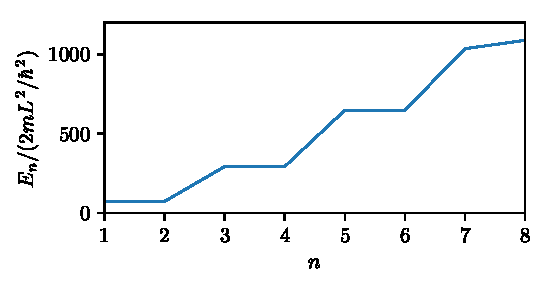
\includegraphics{figs/double_eigenvalues.pdf}%
\caption{Eigenfunctions (top) and eigenvalues (bottom) in a double well with $\Delta x' = 1/1000$ and $\nu_0 = 1000$. The middle barrier is indicated by the central gray area. \label{fig:well_solutions}}%
\end{figure}

The first 6 eigenvalues are given below. We see that the first excited state ($\lambda_2$) is \emph{nearly} degenerate with the ground state ($\lambda_1$), and similarly for $\lambda_3$ and $\lambda_4$, and $\lambda_5$ and $\lambda_6$. The states are not fully degenerate because we cannot have degeneracy in a 1D system like this.
\begin{center}
\begin{tabular}{ccc}
% \hline
$\lambda_1$ = 73.8663877 & $\lambda_2$ = 293.2169877 & $\lambda_4$ = 647.6674955 \\
$\lambda_2$ = 73.8683378 & $\lambda_3$ = 293.2410202 & $\lambda_5$ = 648.1536705
% \\\hline
\end{tabular}
\end{center}

In \cref{fig:double_well_solutions} plots of the probability density is given. We see that the probability density is concentrated the left side of the barrier at $t'=0$, and that it tunnels through the barrier and is fully concentrated on the right side of the barrier at $T = t' = \pi/(\lambda_2 - \lambda_1)$. The tunnelling time $T$ is the (half) period of the exponential of \cref{eq:time_evolution_expansion}.
\begin{figure}[ht!]%
\centering%
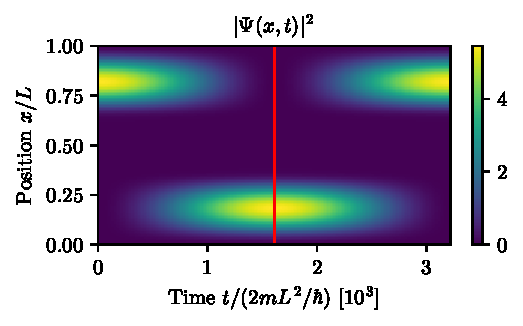
\includegraphics{figs/double_twopsi_prob.pdf}\\%
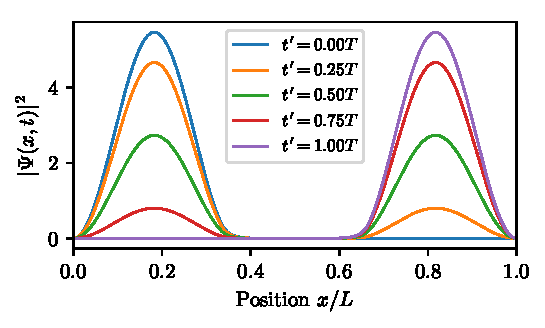
\includegraphics{figs/double_twopsi_prob_1d.pdf}%
\caption{Time evolution of the double well with initial condition $\Psi_0 = 1/\sqrt(2)(\psi_1 + \psi_2)$, $\Delta x' = 1/1000$ and $\nu_0 = 1000$. $T$ is the tunnelling time $t' = \pi/(\lambda_2 - \lambda_1)$, and is indicated by the red vertical line in the top figure. \label{fig:double_well_solutions}}%
\end{figure}

\subsubsection*{Root-finding}
It can be shown that the eigenvectors of the Hamiltonian with energies $0 < \lambda < \nu_0$ are given by the equation
\begin{align}
    f(\lambda) = 
    &e^{\kappa/3}\sbr{\kappa\sin\del{\frac{k}{3}} + k\cos\del{\frac{k}{3}}}^2 \nonumber\\
    & - e^{-\kappa/3}\sbr{\kappa\sin\del{\frac{k}{3}} - k\cos\del{\frac{k}{3}}}^2 = 0,
    \label{eq:roots}
\end{align}
where $k = \sqrt{\lambda}$ and $\kappa = \sqrt{\nu_0 - \lambda}$.

We find the roots of \cref{eq:roots} using the function \pyinline{scipy.optimize.root} from the \python-package \texttt{SciPy}, with the default \verb!hybr! method. This uses a modification of the Powell's hybrid method\cite{powell1970hybrid} implemented in MINPACK’s \verb!hybrd! and \verb!hybrj! routines. Other methods can be selected using the \verb!method! argument, but we found the default method to give sufficient results. We use the eigenvalues $\lambda_1$ to $\lambda_6$ from the previous section as starting points for the function. 

The resulting roots are listed below, and a plot of \cref{eq:roots} with the roots indicated by vertical lines is shown in \cref{fig:roots}. We see that the roots of \cref{eq:roots} doesn't perfectly agree with the eigenvalues found before.

\begin{center}
\begin{tabular}{ccc}
% \hline
$\lambda_1$ = 73.937533 &$\lambda_3$ = 293.516198 &$\lambda_5$ = 648.750278 \\
$\lambda_2$ = 73.935600 &$\lambda_4$ = 293.492315 &$\lambda_6$ = 648.264373
% \\\hline
\end{tabular}
\end{center}

\begin{figure}[ht!]%
\centering%
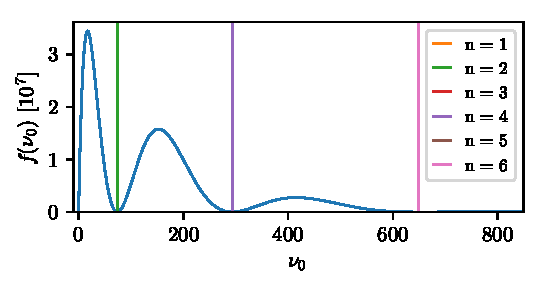
\includegraphics{figs/roots_with_roots.pdf}%
\caption{Plot of \cref{eq:roots}, with the roots indicated by vertical lines. The lines for $n=1$ and $n=2$ overlap, as does $n=3$ and $n=4$ etc. \label{fig:roots}}%
\end{figure}

In \cref{fig:eigenvalues_roots} we have plots of the number of eigenstates with eigenvalues lower than the barrier height $\nu_0$. We find that the barrier height that separates having none and one such eigenstate is approximately $\nu_0 = 22.2$.
\begin{figure}[ht!]%
\centering%
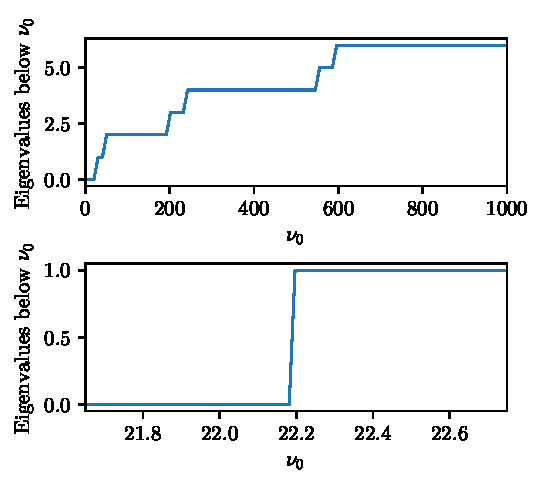
\includegraphics{figs/number_of_roots.pdf}%
\caption{Plots of the number of eigenstates with eigenvalues less than the barrier height $\nu_0$, as function of $\nu_0$. \label{fig:eigenvalues_roots}}%
\end{figure}

\subsection*{Finite difference time evolution}
\begin{itemize}
    % \item \sout{Plot eigenvalues $\lambda_n$ as function of $n$, discuss results}
    % \item \sout{Plot time evolution with tunnelling, discuss tunnelling and why it happens at time $\pi/(\lambda_2 - \lambda_1)$}
    % \item \sout{(Plot $f(\lambda)$ from eq. 3.4?)}
    % \item \sout{Find roots/eigenvalues from eq. 3.4}
    % \item \sout{compare roots to eigenvalues from solving TISE}
    % \item \sout{Estimate barrier height that separates having one eigenstate with $\lambda_n < \nu_0$ and having no such states}
    \item (Plot time evolution using Euler scheme for TISE (eq. 3.6))
    \item Plot time evolution using C-N scheme for TISE (eq. 3.8)
    \item Time-dependent Hamiltonian!! \hl{Discuss when it's advantageous to use step-by-step time evolution. Does it depend on the initial condition? Make a few hypotheses, and test the ideas.}
\end{itemize}

\subsection*{Two-level double well system}

In the left plot in \cref{fig:detuning1} there is a plot of the two lowest eigenvalues $\lambda_1$ and $\lambda_2$ as function of the potential $\nu_r$. In the right plot the two lowest eigenfunctions are plotted for positive and negative $\nu_r$. We see that the ground state $\psi_1$ is localized at the left side for positive $\nu_r$, and mostly located at the right side for negative $\nu_r$, and vice versa for the excited state $\psi_2$.
\begin{figure}[ht!]%
\centering%
% 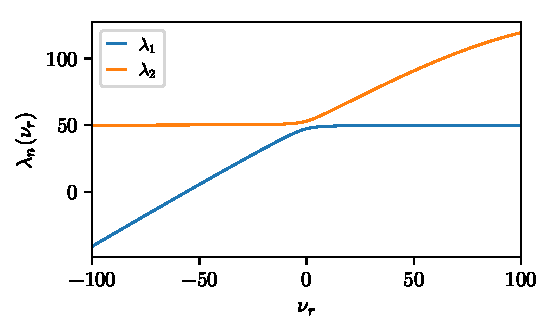
\includegraphics{figs/detuning_4_1.pdf}\\%
% 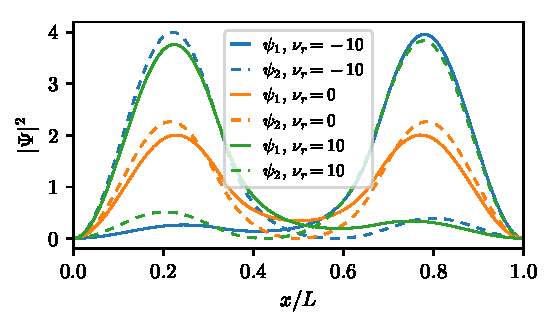
\includegraphics{figs/detuning_localization.pdf}%
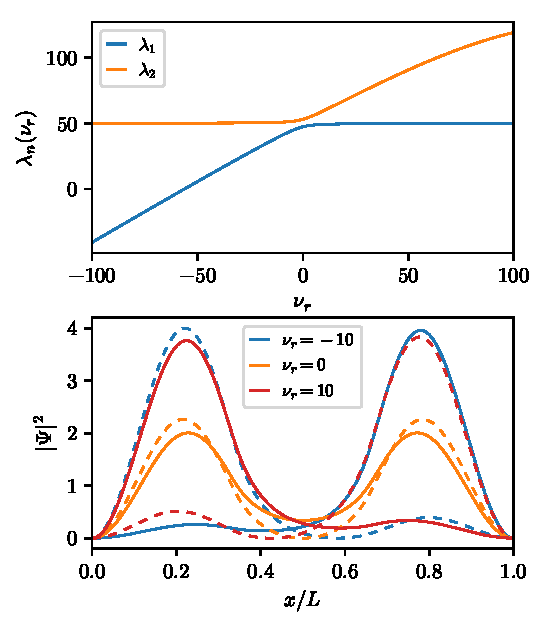
\includegraphics{figs/task4.pdf}%
\caption{(top) Plot of the two lowest eigenvalues as function of $\nu_r$ with $\Delta x' = 1/1000$, and (bottom) localization of ground state with positive and negative $\nu_r$. The solid lines show $\psi_1$ and dashed lines $\psi_2$. \label{fig:detuning1}}%
\end{figure}